\documentclass[conference]{IEEEtran}
% *** GRAPHICS RELATED PACKAGES ***
%
\ifCLASSINFOpdf

\fi
\usepackage{url}
\usepackage[brazilian]{babel}
\usepackage[utf8]{inputenc}
\usepackage[T1]{fontenc}
\usepackage{graphicx}
\usepackage{cite}
\usepackage[pdftex, hidelinks]{hyperref}
\hyphenation{op-tical net-works semi-conduc-tor}

\begin{document}

\title{Simulador de amplificador de áudio}
\author{\IEEEauthorblockN{Paulo Augusto M. F. de Souza}
\IEEEauthorblockA{Estudante de Engenharia Eletrônica\\
Faculdade Gama - FGA UnB\\
Email: pauloaugustomiguelfonseca@gmail.com}
\and
\IEEEauthorblockN{Tiago Martins de Brito}
\IEEEauthorblockA{Estudante de Engenharia Eletrônica\\
Faculdade Gama - FGA UnB\\
Email: tiagomartinsbrito879@gmail.com}
}%final de autores

% make the title area
\maketitle


\begin{abstract}
Com o processamento de sinais de áudio, é possivel modificar as características originais do sinal. Por ser de áudio, pode-se ver o seu comportamento em faixas de frequência diferente e com isso equalizar um sinal da maneira pretendida através de filtros. Também é possível amplificar ele de uma maneira que o torne mais intenso ou menos intenso, modificando a sua amplitude.
\end{abstract}


{\small \textbf{{\textit Palavras-chaves} -- Frequência, filtro, amplificador, equalizador.}}


\IEEEpeerreviewmaketitle



\section{Introdução}
% no \IEEEPARstart
%Equalizar audio, é definir faixas de específicas de frequência.
%Fazer a introdução
 
%\hfill January 11, 2007
\subsection{Justificativa}
Para tratamento de sinais de áudio com equipamentos digitais ou analógicos, ainda há um elevado custo, então como esse projeto tem como motivação tentar reduzir esses custos, mas tendo em vista manter uma certa qualidade. Com esse custo reduzido, poderia ser usado para o aprendizado para quem ainda está aprendendo e não quer gastar muito com equipamentos de áudio. 

\subsection{Objetivos}
O objetivo deste trabalho, é mostrar como pode ser feita a equallização de áudio, com o Raspberry Pi através da amostragem de um sinal. 

\subsection{Requisitos}
A priori está sendo estudada a possibilidade de usar um conversor AD, de pelo menos 16 bits e uma frequência de amostragem de 40kHz, ou no lugar dele colocar uma interface de áudio, que tem uma taxa de amostragem de 48kHz e de 24 bits. Isso se deve pois o Raspberry não possui conversor AD, então é preciso usar um externo. 

Sensores serão usados para colocar algum tipo de efeito durante o processamento do sinal pelo Raspberry, como por exemplo um sensor de distância para colocar a intensidade do efeito. Também pode ser adicionado um VU-Meter, para mostrar as bandas de frequência do sinal. 

Para todos os cálculos e processamentos dos sinais, será usado o Raspberry Pi 3. Ele será usado pois, tem uma grande capacidade de processamento, e com uma boa velocidade. O uso dele permite criar sistemas embarcados para essa aplicação de processamento de sinais de áudio.


\section{Revisão Bibliográfica}
\subsection{Teorema da amostragem}
Para o processamento computacional de um sinal analógico, antes é preciso fazer a amostragem do sinal. Isso consiste em discretizar o sinal, ou seja, torna-lo digital e com isso fazer o seu processamento em um computador, ou no Raspberry Pi. Amostrar é definir para um certo intervalo de tempo, um valor para o sinal. Onde esse ele apenas possui um valor definido em um intervalo de tempo específico.

\begin{figure}[!h]%h = here
\centering

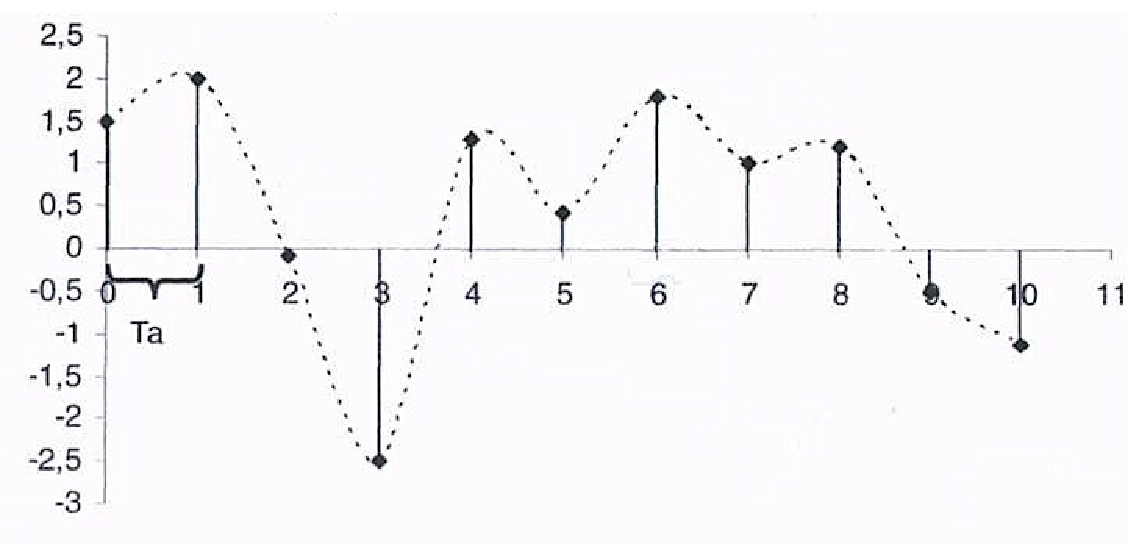
\includegraphics[width=2.5in]{Imagens/amostragem1} %define a largura como 2.5 polegagas
\caption{Amostragem}
%\flushleft{\small 
%Fonte: \url{https://susanasousa.wordpress.com/2011/01/23/audio-digital-frequencia-de-amostragem}}

\label{amos}
\end{figure}

Na Figura \ref{amos}, é possível ver justamente, onde para cada intervalo de tempo é que se tem uma amostra do sinal, um valor definido apenas em um intervalo de tempo específico. Em intervalos de tempo não definido, o sinal recebe zero como seu valor.

Um meio para as discretização, é usar o critério de Nyquist para amostragem, que diz que a frequência de amostragem deve ser de pelo menos duas vezes a frequência do sinal. Isso se deve para que se possa retomar o sinal original com o mínimo de distorções possíveis. 
Na Figura \ref{fig_sim} é possivel ver justamente esse critério, pois quando a frequência de amostragem é duas vezes menor, há uma sobreposição do sinal, e isso não permite voltar ao sinal original. \cite{Linhares:1968}

\begin{figure}[!htb]
\centering
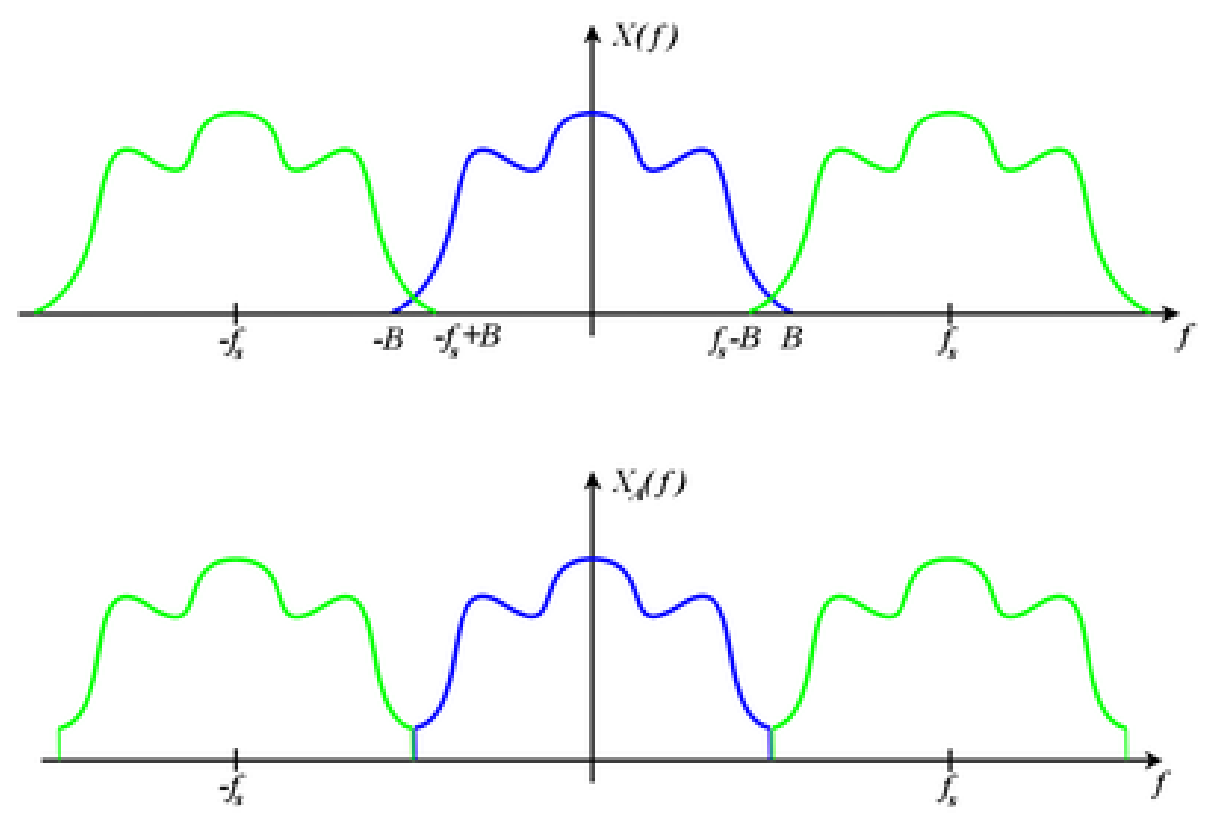
\includegraphics[width=2.2in, height = 1.2in]{Imagens/nyquist}
\caption{Nyquist}
\flushleft{\small 
Fonte: \url{https://pt.wikipedia.org/wiki/Teorema_da_amostragem_de_Nyquist-Shannon}}

\label{fig_sim}
\end{figure}

\subsection{Processamento de sinais}

Em áudio a largura de banda corresponde ao espectro audível, compreendido entre 20 e 20kHz. %citação aqui ppgee.ufmg.br/defesas/486M-PDF
\cite{Linhares:1968}
Então, a partir de dispositivos de captação sonora, o objetivo é trabalhar com faixas de frequência compreendidas na parte audível. Com isso, se busca então trabalhar com a resposta em frequência dessa faixa.

O processamento desses sinais, podem ser feitos com a aplicação de filtros, que delimitam uma faixa específica para se trabalhar. Esses filtros, que podem ser, passa baixas, passa altas ou passa bandas, servem para fazer a equalização de um sinal de áudio. Além dessa equalização, também podem ser incorporados controles para ajuste da amplitude dos sinais antes e após o processamento.

Filtros passa baixas, são dispositivos que permitem a passagem de um sinal até uma certa frequência máxima. Passa altas, são os que permitem a passagem a partir de uma frequência mínima. E passa bandas, são os que permitem a passagem a partir de uma frequência mínima até uma máxima. As figuras abaixo mostram justamente a resposta em frequência de cada filtro.

%%%%%%%%%%%%%%%%%%%%%%%%%%%%%%%%%%%%%%%%%%%%%%

%imagens de filtros
%Passa-Baixas
\begin{figure}[!h]
\centering
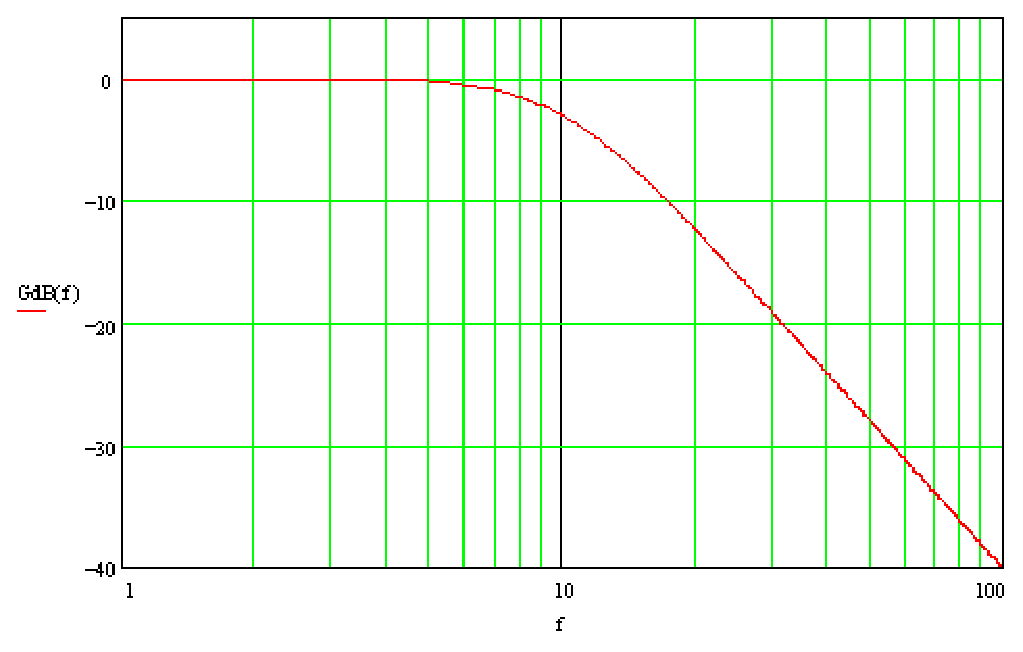
\includegraphics[width=2.5in, height=1.1in]{Imagens/baixass.eps}
\caption{Passa baixas} 
\flushleft{\small 
Fonte: \url{http://www.alvaroneiva.site.br.com/filteq2_arquivos/image011.gif}}
\label{baixa}
\end{figure}
%Passa-Bandas
\begin{figure}[!htb]
\centering
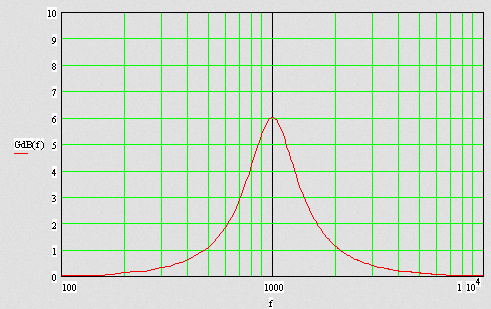
\includegraphics[width=2.5in, height=1.1in]{Imagens/BANDAA.png}
\caption{Passa banda}
\flushleft{\small 
Fonte: \url{http://www.alvaroneiva.site.br.com/filteq2_arquivos/image015.gif}}
\label{banda}
\end{figure}
%Paassa-Altas
\begin{figure}[!htb]
\centering
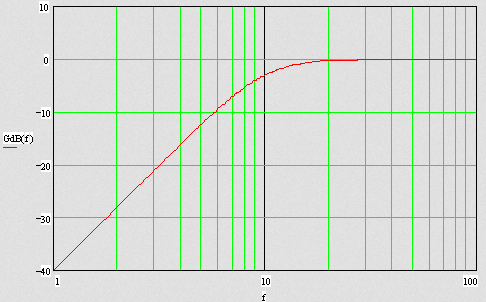
\includegraphics[width=2.5in, height=1.1in]{Imagens/ALTAA.png}
\caption{Passa alta} 
\flushleft{\small 
Fonte: \url{http://www.alvaroneiva.site.br.com/filteq2_arquivos/image013.gif}}
\label{alta}
\end{figure}

\bibliographystyle{plain}

\bibliography{Referencias}


% that's all folks
\end{document}


\grid
